\documentclass[10pt]{article}
\usepackage[letterpaper,textwidth=7.16in,top=0.55in,bottom=0.55in]{geometry}
\usepackage[T1]{fontenc}
\usepackage{lmodern,graphicx,booktabs,amsmath,enumitem,caption,float,hyperref}
\hypersetup{hidelinks}
\setlist[itemize]{nosep,leftmargin=1.3em}
\setlength{\parindent}{0pt}
\setlength{\parskip}{5pt}
\renewcommand{\thesection}{\Roman{section}}
\renewcommand{\thesubsection}{\Alph{subsection}}
\renewcommand{\thetable}{\Roman{table}}
\captionsetup{font=small,labelfont=bf}
\title{NeST-Com: Fixed-Budget Next-Scale Token Communication}
\author{WCL revision outline --- paragraph tasks, not full paper prose}
\date{21 October 2026}
\begin{document}
\maketitle
\textbf{Version boundary.} Frozen main evidence is based on commit \texttt{a5f8ceb0233b0e1f599ee8bb902c1a094d47119d}. The completed ARPC decoding-sensitivity study is a separate matched100 analysis. It does not replace the common500 curves. This one-column file is an editable outline skeleton; the figures are exported at their final 7.16-inch print width.
\section{Introduction}
\begin{itemize}
\item Establish per-image fixed complex-symbol-budget communication and the tradeoffs among pixel fidelity, perceptual similarity, semantic feature consistency, and processing cost.
\item Position continuous JSCC, learned token communication, and digital separation. Ada-TokenCom already combines autoregressive tokens, arithmetic coding, prefix transmission and generation, with rate/MCS adaptation. Briefly mention TONIC's task-oriented token protection and completion. Restrict the gap to next-scale multiscale endpoint granularity under a hard per-image budget.
\item Present within-scale endpoints, actual terminated-length adaptation and prefix-constrained reconstruction as one complete method. Use WHOLE/PARTIAL to examine the mechanism and five methods to evaluate the system; avoid universal superiority or priority claims.
\end{itemize}
\section{Proposed NeST-Com Framework}
\subsection{System Model and Multiscale Representation}
\begin{itemize}
\item Define the frozen tokenizer, multiscale discrete tokens, shared VAR prior and image decoder $D_c$. At $N=1024$, account for 68 header and 956 body complex symbols over AWGN with nominal $E_s=2$.
\item Distinguish complete scales $1,\ldots,m$ from the first $K$ raster-order positions in the next scale. Receiver inputs are actual paid information and shared models, with no source truth or unsent tokens.
\end{itemize}
\begin{figure}[H]\centering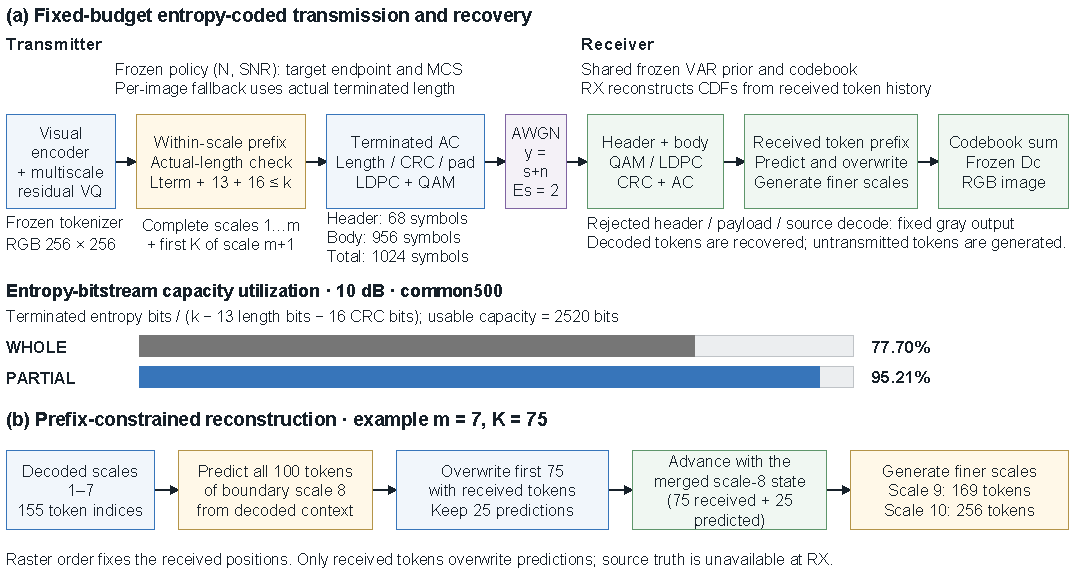
\includegraphics[width=\linewidth]{images/figure1.pdf}\caption{Fixed-budget NeST-Com. Actual terminated arithmetic-code length controls per-image endpoint fallback. At the receiver, transmitted tokens are entropy-decoded; the boundary scale is predicted and received positions are overwritten before finer-scale generation. Entropy-bitstream capacity utilization is reported in Table~\ref{tab:within-scale}; the bird thumbnails are schematic. The $m=7,K=75$ example illustrates the mechanism rather than a universal endpoint.}\label{fig:system}\end{figure}
\subsection{Budget-Adaptive Within-Scale Prefix Transmission}
\begin{itemize}
\item Describe the implemented endpoint set, frozen SNR-specific target/MCS policies and actual fallback order. Do not infer a new policy from test performance. Retain the T1-C m10 correction at 19 dB.
\item Include actual arithmetic termination in $L_{\rm term}+13+16\leq k$. Define entropy-bitstream capacity utilization as $L_{\rm term}/(k-13-16)$, not a token count or spectral efficiency. Keep rejected/no-fit outcomes in the denominator.
\end{itemize}
\subsection{Prefix-Constrained Reconstruction}
\begin{itemize}
\item Explain entropy restoration of sent tokens, prediction of the boundary scale, overwrite of received positions, advancement with the merged state, and generation of finer scales. Aggregate codebook representations and apply frozen $D_c$.
\item State the actual generation seed, sampling and rejection behavior. Separate source decoding from generating missing content. No receiver correction from hidden TX truth is allowed.
\end{itemize}
\section{Experimental Results}
\subsection{Experimental Setup}
\begin{itemize}
\item Five frozen methods: entropy-coded NeST-Com, final 100k Latent JSCC, final adapted 200k SwinJSCC, adaptive BPG + LDPC and adapted ARPC + LDPC. Main population is common500, $N=1024$, SNR 4/10/19 dB.
\item Average three original noises per source, then weight 500 sources equally. Reuse pointwise 95\% source-bootstrap intervals. Source-paired differences are the comparison unit; cross-method noise samples are not identical.
\item LPIPS uses AlexNet. CLIP-I is OpenAI CLIP ViT-L/14 image--image cosine with frozen floating preprocessing and FP32 inference at 224-pixel input. Do not convert it to a percentage or call it CLIPScore. Retain all eight metrics in the archive.
\end{itemize}
\subsection{Comparison With Existing Methods}
\begin{figure}[H]\centering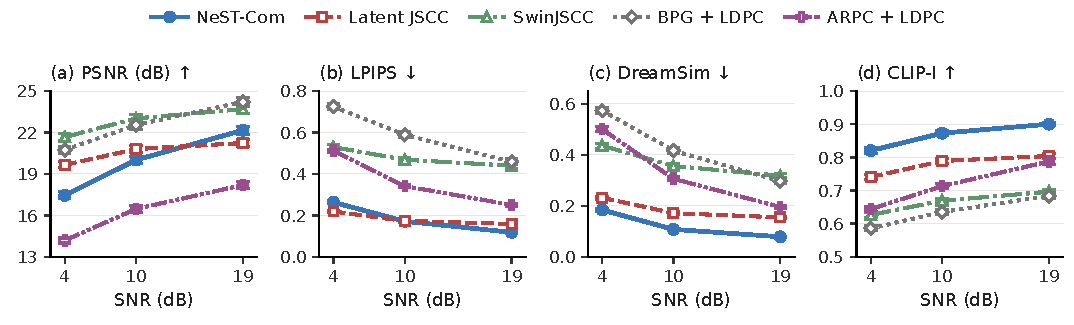
\includegraphics[width=\linewidth]{images/figure2.pdf}\caption{Five-method common500 comparison at $N=1024$. Markers and error bars are frozen means and pointwise 95\% source-bootstrap intervals. Higher PSNR and CLIP-I and lower LPIPS-Alex and DreamSim are favorable. Each source is averaged over three original noise realizations; the 19 dB NeST-Com curve includes T1-C m10 correction.}\label{fig:main}\end{figure}
\begin{itemize}
\item Discuss pixel fidelity, perceptual distances and semantic feature consistency separately. NeST is not best in PSNR at every operating point, and its 4 dB LPIPS is worse than Latent JSCC. LPIPS and DreamSim can disagree. Do not infer significance from marginal CI overlap or attribute CLIP differences to caption conditioning without an ablation.
\item Use the two fixed development cases in Fig.~\ref{fig:examples} to describe visible contours, textures and cart geometry. Do not generalize selected examples to population statistics.
\end{itemize}
\begin{figure}[H]\centering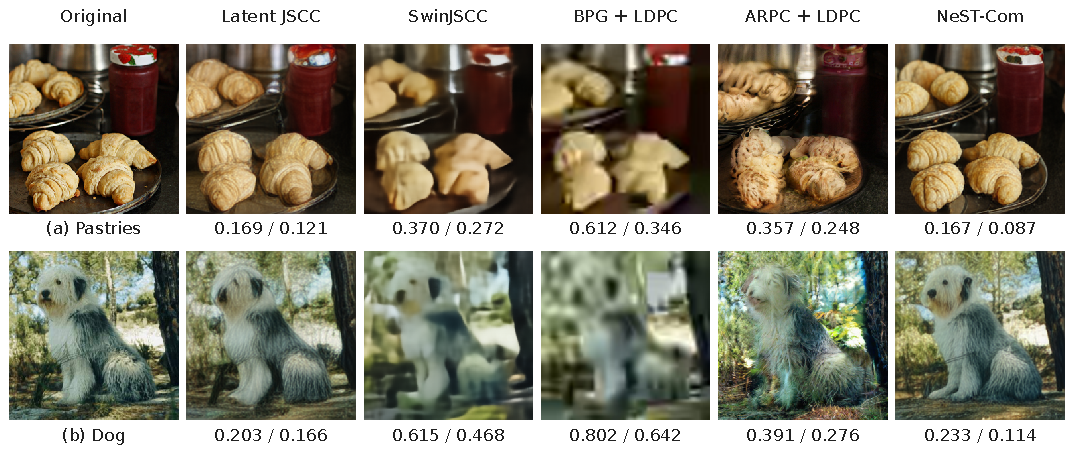
\includegraphics[width=\linewidth]{images/figure3.pdf}\caption{Previously selected Pastries95 and Shopping cart75 development examples at $N=1024$, 10 dB. Full views are retained. Numbers are whole-image LPIPS-Alex / DreamSim for the displayed single reconstruction; both are lower-is-better. Existing LPIPS scores are retained; DreamSim uses the frozen ensemble with FP32 224-pixel bicubic-antialias float preprocessing. Scores correspond to the saved native float arrays.}\label{fig:examples}\end{figure}
\textbf{ARPC decoding sensitivity (completed).} Reuse the same 900 matched100 received events; compare original sampling $\tau=0.5$, explicit argmax, and predeclared $\tau=0.25$ only for untransmitted scales. The two new settings required 592 unique reconstructions, zero new channel events or source encodes, and reused the existing 10,000-resample bank. At 19 dB both alternatives improve all four metrics with favorable paired intervals excluding zero; greedy gives $\Delta$PSNR $=+0.150\,[0.087,0.207]$ dB and $\Delta$DreamSim $=-0.0143\,[-0.0206,-0.0084]$. At 4 dB both worsen LPIPS and DreamSim. At 10 dB only low-temperature PSNR/LPIPS intervals exclude zero favorably; all greedy intervals cross zero. Report all settings and retain original common500 curves. Full results are in \texttt{sensitivity/REPORT.md}.
\subsection{Effect of Within-Scale Endpoints}
\begin{itemize}
\item Use Table~\ref{tab:within-scale} to connect finer legal endpoint granularity to measured loading and quality. At 10 dB utilization increases from 77.70\% to 95.21\% using terminated entropy bits divided by usable source capacity.
\item Define $\Delta=\mathrm{PARTIAL}-\mathrm{WHOLE}$. Report all three PSNR gains and DreamSim reductions with direct paired intervals. Do not treat source-utilization percentiles as confidence intervals on a mean.
\end{itemize}
% Requires booktabs. Values and intervals read from frozen CSV.
\begin{table}[t]
\centering
\caption{Effect of within-scale endpoints at $N=1024$.}
\label{tab:within-scale}
\begingroup
\fontsize{8}{9.5}\selectfont
\setlength{\tabcolsep}{3pt}
\begin{tabular}{@{}r r r c c@{}}
\toprule
SNR & \shortstack{WHOLE\\util. (\%)} & \shortstack{PARTIAL\\util. (\%)} & \shortstack{$\Delta$PSNR (dB)\\{[95\% CI]}} & \shortstack{$\Delta$DreamSim\\{[95\% CI]}} \\
\midrule
4 & 73.81 & 93.08 & \shortstack{$0.616$\\[1pt]$[0.564, 0.673]$} & \shortstack{$-0.0207$\\[1pt]$[-0.0233, -0.0183]$} \\[3pt]
10 & 77.70 & 95.21 & \shortstack{$0.701$\\[1pt]$[0.637, 0.766]$} & \shortstack{$-0.0240$\\[1pt]$[-0.0270, -0.0212]$} \\[3pt]
19 & 85.24 & 94.73 & \shortstack{$0.319$\\[1pt]$[0.290, 0.349]$} & \shortstack{$-0.0030$\\[1pt]$[-0.0037, -0.0024]$} \\[3pt]
\bottomrule
\end{tabular}
\endgroup
\par\smallskip
\begin{minipage}{\linewidth}\fontsize{7.5}{9}\selectfont
$\Delta=\mathrm{PARTIAL}-\mathrm{WHOLE}$, common500, three noise realizations per source. Intervals use direct source-paired differences. Utilization is terminated entropy-bitstream length divided by usable source capacity after the 13-bit length and 16-bit CRC fields. Negative $\Delta$DreamSim favors PARTIAL.
\end{minipage}
\end{table}

\subsection{Performance With a Larger Symbol Budget}
\begin{itemize}
\item Table~\ref{tab:larger-budget} uses matched100, $N=2048$, three noises per source and 300/300 delivered events per method/condition. The 4/10 dB adaptive rows and 19 dB full-representation row are distinct configurations.
\item Retain the 19 dB perceptual boundary: $\Delta$DISTS $=+0.0054\,[+0.0024,+0.0086]$ for NeST minus ARPC, favoring ARPC despite NeST's higher PSNR and lower DreamSim. N2048 CLIP was not started.
\end{itemize}
% Requires booktabs. Values and intervals read from frozen CSV.
\begin{table}[t]
\centering
\caption{Paired differences at $N=2048$.}
\label{tab:larger-budget}
\begingroup
\fontsize{8}{9.5}\selectfont
\setlength{\tabcolsep}{3pt}
\begin{tabular}{@{}l c c@{}}
\toprule
Condition & \shortstack{$\Delta$PSNR (dB)\\{[95\% CI]}} & \shortstack{$\Delta$DreamSim\\{[95\% CI]}} \\
\midrule
4 dB adaptive & \shortstack{$3.779$\\[1pt]$[3.493, 4.082]$} & \shortstack{$-0.2658$\\[1pt]$[-0.2933, -0.2386]$} \\[3pt]
10 dB adaptive & \shortstack{$3.877$\\[1pt]$[3.688, 4.079]$} & \shortstack{$-0.1174$\\[1pt]$[-0.1309, -0.1049]$} \\[3pt]
19 dB full representations & \shortstack{$1.806$\\[1pt]$[1.742, 1.871]$} & \shortstack{$-0.0086$\\[1pt]$[-0.0119, -0.0052]$} \\[3pt]
\bottomrule
\end{tabular}
\endgroup
\par\smallskip
\begin{minipage}{\linewidth}\fontsize{7.5}{9}\selectfont
$\Delta=\mathrm{NeST}-\mathrm{ARPC}$. Matched100, three noise realizations per source, 300/300 delivered frames for each method and condition. The 4/10-dB rows use adaptive endpoints; the 19-dB row uses full representations. Negative $\Delta$DreamSim favors NeST.
\end{minipage}
\end{table}

\subsection{Computational Cost}
% Requires booktabs. Values and intervals read from frozen CSV.
\begin{table}[t]
\centering
\caption{Software processing latency at 10 dB (ms/image).}
\label{tab:latency}
\begingroup
\fontsize{8}{9.5}\selectfont
\setlength{\tabcolsep}{3pt}
\begin{tabular}{@{}l r r r@{}}
\toprule
Method & TX & RX & Total \\
\midrule
NeST-Com & 220.89 & 398.82 & 619.71 \\
Latent JSCC & 17.97 & 24.51 & 42.48 \\
SwinJSCC & 24.81 & 19.89 & 44.69 \\
BPG + LDPC & 2269.87 & 23.15 & 2293.01 \\
ARPC + LDPC & 719.12 & 801.18 & 1520.30 \\
\bottomrule
\end{tabular}
\endgroup
\par\smallskip
\begin{minipage}{\linewidth}\fontsize{7.5}{9}\selectfont
Shared NVIDIA RTX PRO 6000 Blackwell, GPU 1, six CPU cores, batch size 1; 16 fixed development sources, three warmups and three measured repetitions per setting (48 measurements). Total is TX+RX software processing time, excluding air-interface time and model loading. Original method-specific precision is retained; TF32 is off.
\end{minipage}
\end{table}

\begin{itemize}
\item Report existing 10 dB software processing latency: TX, RX and their sum in ms/image. Same registered RTX PRO 6000 Blackwell GPU and six CPU cores, batch one, 16 fixed development images, three warmups and three measurements per source.
\item Retain per-method environments/precision and sampled shared load. Exclude model initialization, AWGN generation, process handoff and audit persistence; include necessary BPG subprocess/file conversion. Do not call these radio or end-to-end network delays or merge historical H800 timings.
\end{itemize}
\section{Conclusion}
\begin{itemize}
\item Summarize the connected endpoint/actual-length/reconstruction design and its observed quality--processing-cost tradeoffs. State low-SNR metric disagreements, decoder sensitivity and full-representation limitations rather than universal superiority.
\end{itemize}
\clearpage
\section*{Related-work source checks}
Ada-TokenCom: \url{https://arxiv.org/abs/2608.28086}. TONIC: \url{https://arxiv.org/abs/2605.21553}. These are related-work context, not additional rerun baselines.
\end{document}
